% Options for packages loaded elsewhere
% Options for packages loaded elsewhere
\PassOptionsToPackage{unicode}{hyperref}
\PassOptionsToPackage{hyphens}{url}
\PassOptionsToPackage{dvipsnames,svgnames,x11names}{xcolor}
% Code above from https://github.com/quarto-dev/quarto-cli/blob/main/src/resources/formats/pdf/pandoc/passoptions.latex
% Customization below
\PassOptionsToPackage{babel}{csquotes}
%
\documentclass[
  french,
  11pt,
]{stylisharticle}
\usepackage{xcolor}
\usepackage{amsmath,amssymb}
\setcounter{secnumdepth}{2}
\usepackage{iftex}
\ifPDFTeX
  \usepackage[T1]{fontenc}
  \usepackage[utf8]{inputenc}
  \usepackage{textcomp} % provide euro and other symbols
\else % if luatex or xetex
  \usepackage{unicode-math} % this also loads fontspec
  \defaultfontfeatures{Scale=MatchLowercase}
  \defaultfontfeatures[\rmfamily]{Ligatures=TeX,Scale=1}
\fi
\usepackage{lmodern}
\ifPDFTeX\else
  % xetex/luatex font selection
\fi
% Use upquote if available, for straight quotes in verbatim environments
\IfFileExists{upquote.sty}{\usepackage{upquote}}{}
\IfFileExists{microtype.sty}{% use microtype if available
  \usepackage[]{microtype}
  \UseMicrotypeSet[protrusion]{basicmath} % disable protrusion for tt fonts
}{}
\makeatletter
\@ifundefined{KOMAClassName}{% if non-KOMA class
  \IfFileExists{parskip.sty}{%
    \usepackage{parskip}
  }{% else
    \setlength{\parindent}{0pt}
    \setlength{\parskip}{6pt plus 2pt minus 1pt}}
}{% if KOMA class
  \KOMAoptions{parskip=half}}
\makeatother
% Make \paragraph and \subparagraph free-standing
\makeatletter
\ifx\paragraph\undefined\else
  \let\oldparagraph\paragraph
  \renewcommand{\paragraph}{
    \@ifstar
      \xxxParagraphStar
      \xxxParagraphNoStar
  }
  \newcommand{\xxxParagraphStar}[1]{\oldparagraph*{#1}\mbox{}}
  \newcommand{\xxxParagraphNoStar}[1]{\oldparagraph{#1}\mbox{}}
\fi
\ifx\subparagraph\undefined\else
  \let\oldsubparagraph\subparagraph
  \renewcommand{\subparagraph}{
    \@ifstar
      \xxxSubParagraphStar
      \xxxSubParagraphNoStar
  }
  \newcommand{\xxxSubParagraphStar}[1]{\oldsubparagraph*{#1}\mbox{}}
  \newcommand{\xxxSubParagraphNoStar}[1]{\oldsubparagraph{#1}\mbox{}}
\fi
\makeatother


\usepackage{longtable,booktabs,array}
\newcounter{none} % for unnumbered tables
\usepackage{calc} % for calculating minipage widths
% Correct order of tables after \paragraph or \subparagraph
\usepackage{etoolbox}
\makeatletter
\patchcmd\longtable{\par}{\if@noskipsec\mbox{}\fi\par}{}{}
\makeatother
% Allow footnotes in longtable head/foot
\IfFileExists{footnotehyper.sty}{\usepackage{footnotehyper}}{\usepackage{footnote}}
\makesavenoteenv{longtable}
\usepackage{graphicx}
\makeatletter
\newsavebox\pandoc@box
\newcommand*\pandocbounded[1]{% scales image to fit in text height/width
  \sbox\pandoc@box{#1}%
  \Gscale@div\@tempa{\textheight}{\dimexpr\ht\pandoc@box+\dp\pandoc@box\relax}%
  \Gscale@div\@tempb{\linewidth}{\wd\pandoc@box}%
  \ifdim\@tempb\p@<\@tempa\p@\let\@tempa\@tempb\fi% select the smaller of both
  \ifdim\@tempa\p@<\p@\scalebox{\@tempa}{\usebox\pandoc@box}%
  \else\usebox{\pandoc@box}%
  \fi%
}
% Set default figure placement to htbp
\def\fps@figure{htbp}
\makeatother


% definitions for citeproc citations
\NewDocumentCommand\citeproctext{}{}
\NewDocumentCommand\citeproc{mm}{%
  \begingroup\def\citeproctext{#2}\cite{#1}\endgroup}
\makeatletter
 % allow citations to break across lines
 \let\@cite@ofmt\@firstofone
 % avoid brackets around text for \cite:
 \def\@biblabel#1{}
 \def\@cite#1#2{{#1\if@tempswa , #2\fi}}
\makeatother
\newlength{\cslhangindent}
\setlength{\cslhangindent}{1.5em}
\newlength{\csllabelwidth}
\setlength{\csllabelwidth}{3em}
\newenvironment{CSLReferences}[2] % #1 hanging-indent, #2 entry-spacing
 {\begin{list}{}{%
  \setlength{\itemindent}{0pt}
  \setlength{\leftmargin}{0pt}
  \setlength{\parsep}{0pt}
  % turn on hanging indent if param 1 is 1
  \ifodd #1
   \setlength{\leftmargin}{\cslhangindent}
   \setlength{\itemindent}{-1\cslhangindent}
  \fi
  % set entry spacing
  \setlength{\itemsep}{#2\baselineskip}}}
 {\end{list}}
\usepackage{calc}
\newcommand{\CSLBlock}[1]{\hfill\break\parbox[t]{\linewidth}{\strut\ignorespaces#1\strut}}
\newcommand{\CSLLeftMargin}[1]{\parbox[t]{\csllabelwidth}{\strut#1\strut}}
\newcommand{\CSLRightInline}[1]{\parbox[t]{\linewidth - \csllabelwidth}{\strut#1\strut}}
\newcommand{\CSLIndent}[1]{\hspace{\cslhangindent}#1}

\ifLuaTeX
\usepackage[bidi=basic,shorthands=off]{babel}
\else
\usepackage[bidi=default,shorthands=off]{babel}
\fi
\ifLuaTeX
  \usepackage{selnolig} % disable illegal ligatures
\fi


\setlength{\emergencystretch}{3em} % prevent overfull lines

\providecommand{\tightlist}{%
  \setlength{\itemsep}{0pt}\setlength{\parskip}{0pt}}



 

\usepackage[]{csquotes}

% -------------- Additional packages
\usepackage{orcidlink}  % Orcid logo and link to author page

% -------------- Font size
% R output: footnotesize
\makeatletter
\patchcmd{\@verbatim}
  {\verbatim@font}
  {\verbatim@font\footnotesize}
  {}{}
% References font size whether bibtex is used or not
\@ifundefined{bibfont}
  {%
    \AtBeginEnvironment{CSLReferences}{\footnotesize}
  }
  {%
    \renewcommand*{\bibfont}{\footnotesize}
  }%
\makeatother

% -------------- longtable 2 columns
% https://tex.stackexchange.com/questions/161431/how-to-solve-longtable-is-not-in-1-column-mode-error
\makeatletter
\let\oldlt\longtable
\let\endoldlt\endlongtable
\def\longtable{\@ifnextchar[\longtable@i \longtable@ii}
\def\longtable@i[#1]{
\begin{figure}[t]
\onecolumn
\begin{minipage}{0.5\textwidth}\scriptsize
\oldlt[#1]
}
\def\longtable@ii{
\begin{figure}[t]
\onecolumn
\begin{minipage}{0.5\textwidth}\scriptsize
\oldlt
}
\definecolor{red}{RGB}{255, 0, 0}
\definecolor{green}{RGB}{0, 255, 0}
\definecolor{blue}{RGB}{0, 0, 255}
\definecolor{grey}{RGB}{191, 191, 191}
\makeatletter
\@ifpackageloaded{caption}{}{\usepackage{caption}}
\AtBeginDocument{%
\ifdefined\contentsname
  \renewcommand*\contentsname{Table des matières}
\else
  \newcommand\contentsname{Table des matières}
\fi
\ifdefined\listfigurename
  \renewcommand*\listfigurename{Liste des Figures}
\else
  \newcommand\listfigurename{Liste des Figures}
\fi
\ifdefined\listtablename
  \renewcommand*\listtablename{Liste des Tables}
\else
  \newcommand\listtablename{Liste des Tables}
\fi
\ifdefined\figurename
  \renewcommand*\figurename{Figure}
\else
  \newcommand\figurename{Figure}
\fi
\ifdefined\tablename
  \renewcommand*\tablename{Table}
\else
  \newcommand\tablename{Table}
\fi
}
\@ifpackageloaded{float}{}{\usepackage{float}}
\floatstyle{ruled}
\@ifundefined{c@chapter}{\newfloat{codelisting}{h}{lop}}{\newfloat{codelisting}{h}{lop}[chapter]}
\floatname{codelisting}{Listing}
\newcommand*\listoflistings{\listof{codelisting}{Liste des Listings}}
\makeatother
\makeatletter
\makeatother
\makeatletter
\@ifpackageloaded{caption}{}{\usepackage{caption}}
\@ifpackageloaded{subcaption}{}{\usepackage{subcaption}}
\makeatother
\usepackage{bookmark}
\IfFileExists{xurl.sty}{\usepackage{xurl}}{} % add URL line breaks if available
\urlstyle{same}
% fallback for those not using the hyperref driver hyperxmp:
\makeatletter
\@ifundefined{xmpquote}{\newcommand{\xmpquote}[1]{#1}}{}
\makeatother
\hypersetup{
  pdftitle={Demo Stylish Article},
  pdfauthor={Lyz PASQUET},
  pdflang={fr-FR},
  pdfkeywords={\xmpquote{template}, \xmpquote{demo}},
  colorlinks=true,
  linkcolor={blue},
  filecolor={Maroon},
  citecolor={Blue},
  urlcolor={blue},
  pdfcreator={LaTeX via pandoc}}


% Set up hyperref, after loading it
\hypersetup{
  linkcolor=black,
  citecolor=black,
  colorlinks=true
}

% Journal information
  \JournalInfo{Publication reference}

% Additional notes (e.g. copyright, DOI, review/research article)
  \Archive{DOI: xxx/xx}

% Article title
\PaperTitle{Demo Stylish Article}

% Authors
\Authors{
      {Lyz PASQUET}%
    \textsuperscript{%
      %
      1%
      %
    }%
    }

% Affiliations
    \affiliation{%
      \textsuperscript{1}%
      AgroParisTech Montpellier%
      , Master 2 BioGET%
      %
      , Somewhere%
      , Montpellier%
      %
      , France%
      , 34000%
      %
    }

% Corresponding author
  %

% Keywords
\Keywords{template, demo}
\newcommand{\keywordname}{Keywords} % Defines the keywords heading name

%	Abstract
\Abstract{
  This document is only a demo explaining how to use the Stylish Article
  template.
}
\begin{document}
% Makes all text pages the same height
\flushbottom

% Print the title and abstract box
\maketitle

% Print the contents section
\tableofcontents

% Remove page numbering from the first page
\thispagestyle{empty}

\section{Introduction}\label{introduction}

\begin{itemize}
\tightlist
\item
  La question de la diversité des forêts tropicales fascine les
  écologues parce qu'elle a des enjeux très importants ({Gibson et al.}
  2011). est qu'elle est difficile à comprendre (Wright 2002).
\item
  Des modèles ont été publiés ({Liang et al.} 2022).
\item
  A l'heure des menaces sur la biodiversité ({Fadrique et al.} 2026),
  une connaissance plus détaillée de la diversité des forêts très
  étudiées est utile.
\end{itemize}

\section{Matériel et méthode}\label{matuxe9riel-et-muxe9thode}

\begin{itemize}
\tightlist
\item
  Comparer la diversité de Paracou (Gourlet-Fleury et al. 2004) et de
  BCI (Raby 2017).
\item
  Les analyses sont réalisées avec R (R Core Team 2026) et le package
  divent (Marcon et Puech under review).
\end{itemize}

\subsection{Présentation du site de
Paracou.}\label{pruxe9sentation-du-site-de-paracou.}

La forêt de Parou est située en Guyane française.

\subsection{Présentation du site de
BCI.}\label{pruxe9sentation-du-site-de-bci.}

BCI est une forêt secondarisée (Raby 2017).

Les données sont dans le package \emph{vegan} (Oksanen et al. 2012).

Vérification des données : courbe Rang-abondance (Whittaker 1965).

\section{Résultats}\label{ruxe9sultats}

\begin{figure}

\centering{

\pandocbounded{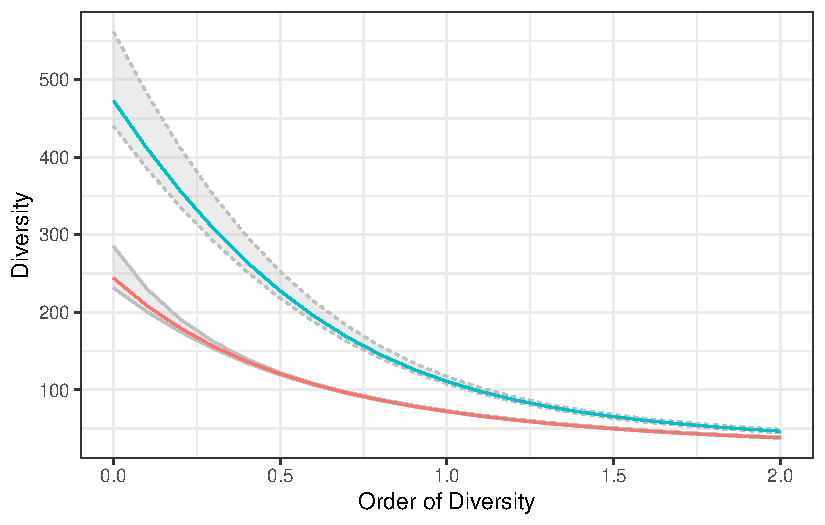
\includegraphics[keepaspectratio]{index_files/figure-pdf/Profils-1.pdf}}

}

\caption{\label{fig-Profils}Profils de diversité de Paracou parcelle 6
et BCI (courbe rouge). La figure représente le nombre effectif d'espèces
(nombre de Hill) en fonction de l'ordre de la diversité.}

\end{figure}%

\section{Discussion}\label{discussion}

\begin{itemize}
\tightlist
\item
  MacArthur et Wilson (1967) montrent mathématiquement que la richesse
  spécifique (le nombre d'espèces) d'une île est un équilibre dynamique
  entre le taux d'immigration et le taux d'extinction, ce dernier étant
  directement dicté par la taille de l'île.
\item
  Sa diversité pourrait être augmentée selon la théorie de la
  perturbation intermédiaire (Connell 1978).
\end{itemize}

\section*{References}\label{bibliography}
\addcontentsline{toc}{section}{References}

\protect\phantomsection\label{refs}
\begin{CSLReferences}{1}{1}
\bibitem[\citeproctext]{ref-Connell1978}
Connell, Joseph H. 1978. {«~Diversity in tropical rain forests and coral
reefs~»}. \emph{Science} 199 (4335): 1302‑10.
\url{https://doi.org/10.1126/science.199.4335.1302}.

\bibitem[\citeproctext]{ref-Fadrique2026}
{Fadrique, B., F. Costa, F. Cuesta, et al.} 2026. {«~Tree diversity is
changing across tropical Andean and Amazonian forests in response to
global change~»}. \emph{Nature Ecology \& Evolution} 10 (2): 267‑80.
\url{https://doi.org/10.1038/s41559-025-02956-5}.

\bibitem[\citeproctext]{ref-Gibson2011}
{Gibson, Luke, Tien Ming Lee, Lian Pin Koh, et al.} 2011. {«~Primary
forests are irreplaceable for sustaining tropical biodiversity~»}.
\emph{Nature} 478 (7369): 378‑81.
\url{https://doi.org/10.1038/nature10425}.

\bibitem[\citeproctext]{ref-Gourlet-Fleury2004}
Gourlet-Fleury, Sylvie, Jean Marc Guehl, et Olivier Laroussinie. 2004.
\emph{Ecology \& management of a neotropical rainforest. Lessons drawn
from Paracou, a long-term experimental research site in French Guiana}.
Elsevier.

\bibitem[\citeproctext]{ref-Liang2022}
{Liang, Jingjing, Javier G. P. Gamarra, Nicolas Picard, et al.} 2022.
{«~Co-limitation towards lower latitudes shapes global forest diversity
gradients~»}. \emph{Nature Ecology \& Evolution} 6 (août): 1423‑37.
\url{https://doi.org/10.1038/s41559-022-01831-x}.

\bibitem[\citeproctext]{ref-MacArthur1967}
MacArthur, Robert H., et Edward O. Wilson. 1967. \emph{The theory of
island biogeography}. Monographs in population biology. Princeton
University Press.

\bibitem[\citeproctext]{ref-Marcon2026a}
Marcon, Eric, et Florence Puech. under review. {«~divent: an {R} Package
for Diversity Measures Based on Entropy~»}. \emph{Journal of Open Source
Software}, under review.

\bibitem[\citeproctext]{ref-Oksanen2012}
Oksanen, Jari, F. Guillaume Blanchet, Roeland Kindt, et al. 2012.
\emph{vegan: Community ecology package}.
\url{http://cran.r-project.org/package=vegan}.

\bibitem[\citeproctext]{ref-R}
R Core Team. 2026. \emph{R: A Language and Environment for Statistical
Computing}. R Foundation for Statistical Computing.
\url{https://doi.org/10.32614/R.manuals}.

\bibitem[\citeproctext]{ref-Raby2017}
Raby, Megan. 2017. \emph{American tropics: the Caribbean roots of
biodiversity science}. Flows, migrations, et exchanges. The University
of North Carolina Press.

\bibitem[\citeproctext]{ref-Whittaker1965}
Whittaker, R. H. 1965. {«~Dominance and diversity in land plant
communities~»}. \emph{Science} 147 (3655): 250‑60.
\url{https://doi.org/10.1126/science.147.3655.250}.

\bibitem[\citeproctext]{ref-Wright2002b}
Wright, S. Joseph. 2002. {«~Plant diversity in tropical forests: a
review of mechanisms of species coexistence~»}. \emph{Oecologia} 130
(1): 1‑14. \url{https://doi.org/10.1007/s004420100809}.

\end{CSLReferences}




\end{document}
